\documentclass[]{vldb}
\usepackage{graphicx}
\usepackage{times}
%\usepackage[T1]{fontenc} 
%\usepackage{tgtermes} 
\usepackage{amsmath}
\usepackage{verbatim}
\usepackage{epsfig}
\usepackage{epstopdf}
%\usepackage{microtype}
%\usepackage[iso]{umlaute}
\usepackage{amssymb}
\usepackage{graphicx}
\usepackage{bbm}
\usepackage{subfigure}
\usepackage{ifthen}
\usepackage{url}
\usepackage{algorithm}
\usepackage{color}
%\usepackage{marginnote}
\usepackage{algorithmic}
\usepackage{paralist}
\usepackage{tabularx}
\usepackage[justification=centering]{caption}
\usepackage[capitalise]{cleveref}

\newcommand{\TODO}[1]{{\bfseries\color{red}TODO: #1}}
\newtheorem{theorem}{Theorem}[section]
\newtheorem{definition}{Definition}
\newtheorem{lemma}{Lemma}
\newtheorem{corollary}{Corollary}
\newtheorem{example}{Example}

\newcommand{\dingedit}[1]{\textcolor{red}{\emph{[Ding: #1]}}}

\title{RideSharing}

\author{}


\begin{document}

\maketitle

\begin{abstract}

\end{abstract}

\section{Introduction}
\label{sec:intro}
%TO-DO lists:
%\begin{itemize}
%	\item Problem definition: define driver profile, rider profile and our price model.
%	
%	\item Define our objective functions (i.e., maximize extra profit), and differentiate it with other optimization goal (e.g., minimize extra distance). 
%	%Given a rider and a driver with their profiles, calculate the cost of accepting the rider. 
%	
%	\item Introduce overall framework, and describe our auction-based mechanism.
%	
%	\item Properties of our framework in both local setting and global setting. In the local setting, show that we will get the same profit as the centralized setting. In the global setting, show that our technique can achieve certain approximation ratio compared with the global optimal (or upper bound of global optimal),  or vice verse we will suffer from certain degenerated cases.
%	
%	\item Optimizations: a) Maintain coarse-grained hierarchic index (adaptive grids, quad-tree), b) maintain novel shortest path index which is fine tuned for ride-sharing applications c) batch processing rider requests (single round bidding v.s. multi-round bidding).
%	
%\end{itemize}

%%%%%% 1. background information
% Ridesharing becomes popular recently because it has potential to match riders with similar itineraries and time schedules, and to bring significant benefits to individual users and the city as a whole. 

Real-time ride-sharing, as an alternative transportation service, alleviates traffic congestion and decreases auto emissions. With the emergence of many commercial platforms (e.g., Uber and Lyft), which automatically match drivers and riders on-the-fly, real-time ride-sharing becomes more and more popular. According to~\cite{uberpool}, millions of trips have been taken on UberPool since its launch at August 2014, and thousands of passengers take it five times a week during commuting hours. Enabled by the development and technology advances of smart phones and location-based services, ride-sharing platforms typically operate as follows: (1) Riders and drivers can join the platform via their smart phones, (2) a rider can submit a request, which consists of the pick-up and drop-off points, to the platform, (3) once a new request is received, the platform determines a driver (even en-route) to pick up the rider, (4) when the trip is completed, the platform calculates the rider's fare and the driver's income. With these platforms, riders can share a vehicle with reduced trip cost while enjoying fast and convenient transportation.

%%%%%% 2. explain the challengs and the detour of ridesharing......
Many challenges exist to enable such real-time ride-sharing platforms. From a business point of view, the platform provider (e.g., Uber) seeks to maximize its own profit. However, higher profits should not be at the cost of either charging passengers more or paying drivers less than what would compromise participation and retention due to no monetarily incentive for either parties. Consequently, the design of a fair pricing model becomes an essential business strategy. This is particularly important in cases of carpooling where riders share their ride with other riders. Even though carpooling reduces the riders' cost, it incurs extra distance (i.e., detour) for riders. While each rider's fare should be discounted as a function of the length of the detour, the driver should be rewarded more as the total travel distance is increased due to all detours. Furthermore, different users (i.e., riders and drivers) might value their time differently. Therefore, a fair pricing model should be available to both riders and drivers to express, for a certain amount of detour, how much discount or compensation they expect. Finally, in addition to fair pricing scheme for riders and drivers, the model should account for the provider's revenue as well.

The second challenge of a ride-sharing platform is to process incoming requests in real-time. This involves two different tasks: i) checking which drivers can add the new requests (new pick-up and drop-off locations) to their current trip without violating the constraints of that trip (i.e., scheduling) and ii) selecting the best driver among those who can serve the new request (i.e., matching). Processing the schedule of potentially thousands of drivers to check if they can accommodate a new request, with the additional task of matching their pricing profile with the incoming rider's profile, becomes computationally intensive. Therefore, the design of an efficient and scalable algorithm that assigns riders to drivers with a fair pricing model while maximizing the provider's revenue, is very challenging.


%First, the framework should consider the conflicting interests of different users (i.e., riders and drivers) and platform providers (e.g., Uber). For example, riders would like to arrive at their destination as quick and cheap as possible, whereas drivers and platform providers would like to maximize their profits. Although ride-sharing can reduce the cost of riders by sharing similar itineraries, it also incurs extra travel distance (i.e., detour). Ideally, riders are expected to be compensated for their detour, while drivers are expected to earn more profit. These factors makes the design of a fair pricing scheme (i.e., the fares and incomes) that satisfies the requirements of both riders and drivers even more complex. Secondly, because the riders requests are generated on-the-fly, the framework should decide the matching drivers (even en-route) at a short amount of time. Therefore, the design of an efficient framework that match riders and drivers, with a fair pricing scheme that provides incentives for all participants becomes a distinguishing business strategy. 

%%% 3. show the shortcomings of existing work and how they fail to address the challenge
The majority of previous studies~\cite{Ota15, Cici15, Cao15, PelzerITS15} focus on improving the efficiency of on-the-fly assignment with the objective of minimizing the total travel distance of drivers. In particular, in existing studies a new request is assigned to a driver who can fit the request in his schedule with the least amount of increase in the total traveled distance. However, minimizing drivers' total travel distance is not always equivalent to overall shorter trips for riders. Consequently, when assigning a new request, the driver who would incur the minimum increase in total travel distance is not necessarily the most cost effective option. To illustrate, suppose driver $a$ has two passengers on board and driver $b$ has only one. To serve an incoming request, \textit{a}'s incurred detour is 2 miles while for $b$ the detour is 3 miles. Even though $a$'s detour is shorter, the platform owner has to compensate both passengers of $a$ for 2 miles (a total of 4 miles) while in the case of $b$ it has to compensate only one passenger for a total of $3$ miles. In addition, from the riders' perspectives, in the first scenario two riders incur extra detour while in the second only one rider incurs an extra detour.  Few studies~\cite{Ma13,Ma15} consider a pricing model by defining monetary incentives for riders and drivers. In \cite{Ma13}, a pricing model is introduced where instead of being compensated, a rider can potentially end up being penalized for longer detours by paying a higher fare. Ma et. al.~\cite{Ma15} overcomes the unfairness issue in \cite{Ma13} to some extent. Even though, a new rider can incur detour in his trip, their model only compensates riders that are already on board. In addition, since this model is targeted for a different application, the notion of revenue fails to provide any incentive for the platform provider. Furthermore, in all previous studies~\cite{Ma13,Huang14,Ma15}, a centralized server is responsible for matching and scheduling incoming requests. Most of these studies utilize a spatiotemporal index to enable matching, i.e., narrowing down the number of potential drivers who can serve an incoming request. With thousands of drivers in the system, even after applying the spatial index, the centralized server still needs to perform scheduling and profile matching for all the candidate drivers. We show that with large number of drivers, these frameworks fail to process new requests in real-time (\cref{subsec:exprp}) and hence not scalable.


%in In \cite{Ma13}, a pricing model is introduced where instead of being compensated, a rider can potentially end up being penalized for longer detours by paying a higher fare. 

%In a recent study \cite{Ma15}, the pricing model overcomes the unfairness issue in \cite{Ma13} to some extent. Since riders can value their time differently, It also allows riders to accept/reject ride-sharing requests based on the amount they will be compensated for the incurred detour. However, drivers can similarly value their time different from each other. The pricing model in \cite{Ma15} does not provide any means for drivers to specify their monetary expectations for participating in the system. Furthermore, since this model only tends to divide the cost of the ride among riders, the notion of revenue is left out and it does not provide any incentive for the platform provider.


%%% 4. explain our pricing model, and provide more intuition of better service quality.
To address aforementioned challenges, in this paper, we introduce an Auction-based Price-Aware Real-time (\textit{APART}) ride-sharing framework. We propose a general and versatile pricing model that allows both riders and drivers to set their monetary expectations for participating in ride-sharing based on their predefined profiles. Specifically, each rider's profile defines the expected discount ratio for the detours incurred by ride-sharing. For example, one rider can express that he is willing to accept a 10 mile detour for 30\% discount. On the other hand, each driver's profile defines the expected cost in terms of his total travel distance and time. The model also accounts for the revenue of the platform provider. Consequently, our objective is to maximize the revenue of the ride-sharing framework while satisfying various temporal and monetary constraints of all users. APART is price-aware because a new request is assigned to a driver which generates the highest profit. Since our pricing model is designed to compensate riders for detours, the most profitable choice is also the one where \textit{riders} incur the least amount of detour, hence better service quality. Finally, APART also maximizes the revenue of the provider by increasing the service rate (throughput) in the system through engaging available drivers more effectively to serve more requests.


% With our price scheme, our objective is to maximize the total profit of the ridesharing platform, while satisfying the constraints of both riders and drivers.

% Because our pricing model compensates riders for longer trips, in order to maximize the profit, our framework reduces the detour of passengers and hence, providing better service quality. 

%We define a fair price model, which is flexible and general. The profiles are served to xxx. The constraints of are expressed as profiles. Given a user and rider profile, the fare and cost of xxx can be automatically derived from their profiles and other constrains. 

%%% 5. explain our framework
To efficiently assign riders to the candidate drivers, we introduce a distributed auction-based framework. With our framework, APART, the server broadcasts a new request to a set of candidate drivers and the mobile app of each candidate driver\footnote{Hereafter we use the term \qoutes{driver} to refer to both the human driver and the software running on his mobile device.} computes and submits a bid based on the driver's current schedule, his and his other passengers' profiles and other spatiotemporal constraints. Subsequently, the server collects all the bids from candidate drivers and assigns the rider to the highest bidding driver. To guarantee high service quality, each driver runs a branch-and-bound algorithm that performs an exhaustive search to find out whether it can fit a new request into its current scheduling. Each driver carries a small number of riders so even an exhaustive search can be performed in real-time. Due to the distributed nature of APART, all candidate drivers perform the search in parallel. Once each driver finds its own best schedule, the server simply selects the driver that generates the highest profit. Consequently, APART is able to find the most profitable drivers in real-time.


%With APART, the server does not need to know the exact location of every driver as it is not responsible for performing the scheduling phase. The grid index structure in APART, only needs to store which grid cell a driver is located in. Therefore, compared to a spatial index structure where the exact location of every driver is stored, APART's grid index requires fewer updates and less maintenance, which further reduces the load on the server.

%%% 6. show some experiment resutls

We conducted extensive experiments on a large scale New York City taxi dataset and show that APART is scalable and efficient, capable of processing hundreds of tasks per second in the presence of thousands of drivers. By comparing our framework with the state-of-the-art approaches~\cite{Huang14}, we show that our framework can simultaneously match up to 10\% more riders to drivers (i.e. higher service rate), while the total travel distance of riders are 20\% less (i.e., better service quality), hence our framework can generate more profit than other approaches with an even better service quality. On the other hand, we show that in a framework were riders are assigned to drivers with the least increase in the driver's travel distance, up to 25\% of the requests are not assigned to the most profitable driver. 

The remainder of this paper is organized as follows. We define our problem in \cref{sec:problem_def}, and explain our pricing model in \cref{sec:pricing}. We present our APART framework, and discuss its auction-based approach in \cref{sec:framework}. In \cref{sec:exp}, we report the experiment results. We discuss the related work in \cref{sec:related} and conclude the paper in \cref{sec:conclusion}.


%%%%%%%%%%%%%%%%%%%%%%%%%%%%%%%%%%%%%%%%%%%%%%%%%%%%
%%% from mohammod 

% Because platforms like Uber and Lyft are becoming more popular (we can show some numbers how their businesses are growing in the recent years). Ridesharing become popular recently. Existing ridesharing studies mainly focus on matching riders and drivers only considering their spatiotemporal constraints (max wait time, maximum detour, etc.)

% It is important to design systems that not only satisfy spatiotemporal constraints of the users, but also take into consideration the monetary aspect of the business (i.e., the fees riders pay, the drivers' income and the system's profit). A key component of such framework is to xxx and xxx.

% While most studies ignore this aspect of the system, T-Share provides a pricing model where on average riders end up paying less when compared to each passenger riding alone. However, based on some experimental results on NYC's taxi dataset, we noticed based on this pricing model, up to x\% of passengers end up paying even more that what they would have payed if they did not share a ride. Hence, this requires the design of a pricing model which is fair to every passenger meaning that if a passenger's trip gets longer as a result of sharing a ride, they should end up paying less (receiving a discount).

% To address the above challenges, in this paper we propose xxx. The goal of our framework is to maximize the profit of the platform. Because we utilize a pricing model which compensates riders for longer trips, in order to maximize the profit, our framework reduces the detour of passengers and hence, providing better service quality.

% Also, APART utilized an auction based approach allowing it to scale by distributing the computation among drivers (You can probably use a good chunk of this part from my CIKM submission).

% We evaluated our .

% The paper is organized as follows:

\section{Problem Definition}
\label{sec:problem_def}

In this section, we define the terminologies, and formally define the problem under consideration.

\subsection{Basic Concepts}
The road network is represented as a graph $G(V, E)$, where each node represents intersections, and each edge represents a road segment. 
Each edge $(i,j) \in E$ $(i, j \in V)$ is associated with a weight $c(i,j)$ which is a travel cost (can be either time or distance) from $i$ to $j$.
% TODO: define path in road network
The shortest path cost $d(s,t)$ is defined as the minimal cost path connecting $s$ and $t$. With our approach, APART, time and distance can be converted from one to the other.

\begin{definition} [Ride Request]
\label{def:req}
A ride request r can be represented as $\left\langle s, e, w, \epsilon, F \right\rangle$ consisting of a starting point $s \in V$ and an end point $e \in V$. Each request also specifies $w$ as the maximum time the rider can wait after making a request and the maximal detour $\epsilon\cdot d(s, e)$ the rider can afford . In addition, a rider's profile $F: \delta d \rightarrow \left[ 0, 1 \right] $, specifies the relative discount in exchange for an incurred detour of $\delta d$.
%the ridesharing fare she would accept based on the extra detour and the shortest possible trip.
\end{definition}

Upon the acceptance of a request, \fname assigns it to a driver.

\begin{definition} [Driver]
A driver v is represented as $\left\langle L, n, g \right\rangle$ where $L$ is the list of ride requests assigned to $v$, and $n$ is the maximum number of requests v can accept at any point in time. A driver also has a profile $g: d \rightarrow \$ $ which specifies the monetary cost of v driving a distance d while servicing its assigned requests.
\end{definition} 

\begin{definition} [Schedule]
Given a set $L$ with n requests, a schedule $S= \left\langle x_1, \cdots, x_{2n} \right\rangle$ is an ordered sequence of pick-up and drop-off points for these request, where for each $r_i \in L$, $r_i.s$ precedes $r_i.e$ in $S$. 
\end{definition}

A schedule is \textit{valid} for a driver \textit{v}, if it satisfies the following conditions:

\begin{itemize}
\item The riders' waiting time constraint: for any request $r_i$, the waiting time from the time the request is made until $v$ arrives at $r_i.s$ should be less than $r_i.w$.
\item The driver's capacity constraint: the number of riders in the vechile cannot exceed the total capacity $n$.
\item Detour constraint: the maximum distance of every rider's trip should be less than $(1+\epsilon) \cdot d(r_i.s, r_i.e)$.
\item The driver's and all riders' (the new rider and the those already in the vehicle) monetary constraints (See \cref{sec:pricing})
\end{itemize}

The driver follows the sequence of picking up and dropping off riders. The schedule changes over time as riders are serviced (picked-up/dropped-off) and new requests are added to the schedule. In fact, adding a new request to a schedule can re-order some requests that already exist in the schedule. For example, when a new request $r_3$ arrives, the initial schedule of $\left\langle s_1, s_2, e_1, e_2 \right\rangle$ can be reordered to $\left\langle s_1, s_2, s_3, e_2, e_3, e_1 \right\rangle$, where rider 1 is dropped off after rider 2.

\begin{definition} [Matching]
Assuming we have a set of drivers V and a set of requests R, we call $M \subset V \times R$ a matching if for each $r \in R$ there is at most one $v \in V$ such that $\left( v, r \right) \in M$. We call $\left( v, r \right) \in M$ \emph{a match}.
\end{definition}

\noindent In a matching $M$, for every driver $v$, there exists a \textit{valid} schedule $S_v$, such that $(v, r_i) \in M \implies r_i.s \in s_v \wedge r_i.e \in S_v$ (or simply $r_i \in S_v$). 

In \cref{sec:pricing}, we define a generic \textit{pricing model} where given a driver and its schedule, the pricing model computes the final fare each rider has to pay, the income of the driver and the ride-sharing platform's profit. Subsequently, we can define the \textit{ride-sharing} problem as follows:

\begin{definition} [Ride-sharing Problem]
Given a set of ride requests R and a set of drivers V, the goal of the ride-sharing problem is to find a matching M between R and V such that the revenue of M is maximized.
\end{definition}

%\dingedit{Justify that our objective function is different with minimizing the travel cost.} \moedit{If we have space at the end, we can give a simple contrary example to prove this.}

%\subsection{Problem Complexity}

%In this section, we perform a brief complexity analysis of the ride-sharing problem. First we show that the problem is NP-Hard. Subsequently, we define the \textit{online} version of the problem and prove there is no online algorithm that can generate an n-approximation solution for the ride-sharing problem.

%\begin{theorem}
%The Ride-Sharing problem is NP-Hard.
%\end{theorem}

%\begin{proof}
%For a given solution of the ride-sharing problem, one can compute the fare of all riders by finding the shortest possible route for their trips and subsequently, the length of the detour incurred to their route. Similarly, we can find the total traveled distance of the riders and compute their income and hence, compute the revenue of the platform. Therefore, the problem is \textit{verifiable} in polynomial time.\\
%Next, we show that the Vehicle Routing Problem (VRP) \cite{Dantzig59} is reducible to the ride-sharing problem in polynomial time. For that we correspond each node in the VRP problem to a request such that the pick-up location of the request is the location of the node and the drop-off point of the request is the central depot in the VRP problem. We also assume, regardless of their detour, every rider pays a constant $f$ and every driver is rewarded $i$ per unit of length. Assuming there are n nodes in the VRP problem, there is a solution of size $K$ for VRP, if and only if there is a rider to driver matching in the ride-sharing problem that generates a revenue of $n.f - K$. Therefore, VRP is reducible to the ride-sharing problem in polynomial time which concludes the proof.
%\end{proof}

The ride-sharing problem is NP-Hard since the Vehicle Routing Problem (VRP) \cite{Dantzig59} is reducible to the ride-sharing problem in polynomial time. A globally optimal solution to the ride-sharing problem can be achieved when a Clairvoyant exists which knows what requests are going to be submitted to the framework at what time and also has the knowledge of which drivers are going to be available, in advance. However, in this paper we study the \textit{online} version of the problem, i.e., the framework has no knowledge regarding future requests and incoming requests have to be matched with drivers as soon as they are submitted to the framework. The optimality of online algorithms are usually analyzed using \textit{competitive ratio} \cite{Sleator85}, i.e., an algorithm $\mathcal{A}$ is called \textit{c-competitive} for a constant $c > 0$, if and only if, for any input $\mathcal{I}$ the result of $\mathcal{A}(\mathcal{I})$ is at most $c$ times worst than the globally optimal solution. In the following we show no online algorithm can achieve a good competitive ratio for ride-sharing problem.

\begin{theorem}
\label{th:comp_ratio}
There does not exist a deterministic online algorithm for the ride-sharing problem that is \textit{c-competitive} ($c > 0$). 
\end{theorem}

\begin{proof}
Suppose there exists an algorithm $\mathcal{A}$ that is \textit{c-competitive}. We assume there exist a Clairvoyant which knows every decision $\mathcal{A}$ makes. For simplicity, we assume there is only one driver at point $(0, 0)$. The input starts with $r_1$ with a pick-up location at $(w, 0)$ and $r_2$ with pick-up location at $(-w, 0)$ (we assume all requests have a maximum wait time of $w$). The algorithm can make three choices for the driver. (1) move toward $r_1$, (2) move towards $r_2$ and (3) stay still. If choice 1 is selected, the Clairvoyant can generate the input such that at time $t = 1$, $n$ more request are submitted with pick-up location at $(-w-1, 0)$ and drop-off locations similar to $r_2$. Similar arguments can be made if choice 2 or 3 are selected by the algorithm. A globally optimal solution can complete $n+1$ requests while $\mathcal{A}$ can at most complete one request. By adding more drivers far away in a similar situation, the Clairvoyant can make $\mathcal{A}$'s solution unboundedly worse than the optimal solution. Therefore, we contradicted the assumption that $\mathcal{A}$ is \textit{c-competitive}.
\end{proof}

%%% TODO: given a rider and the current schedule, calculate the extra profit of inserting a new request.

%Properties of the above definition, can we guarantee the extra profit should be positive?


\section{System Overview}
Describe the following parts:

\begin{figure}[!ht]
	\centering
	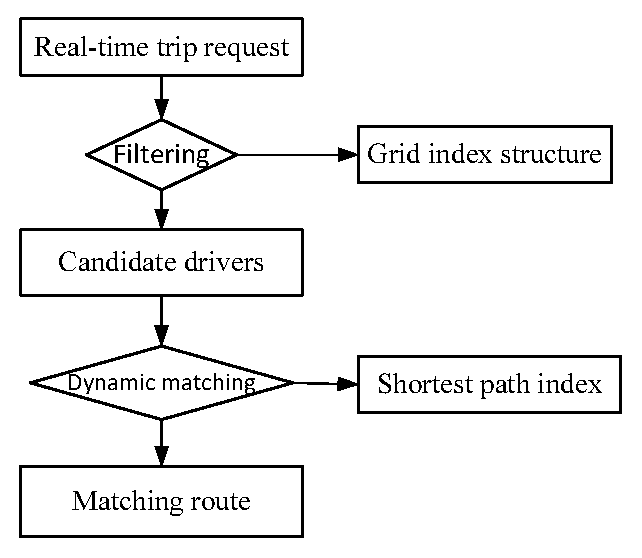
\includegraphics[width = 50mm]{fig/framework.eps}
	\vspace{-0mm}\caption{Framework} \vspace{-2mm} 
\end{figure}\vspace{-0mm}

\begin{itemize}
	\item Overall framework: system components
	\item Explain our auction-based mechanism
	\item Describe the algorithm of inserting a trip requests into a set of driver schedules.
\end{itemize}

\begin{lemma}
	\textbf{In the local setting, The profit through our auction-based mechanism is the same as centralized setting.}
\end{lemma}

\begin{lemma}
	\textbf{In the global setting, show the properties of our auction-based mechanism}
\end{lemma}

Show our auction-based mechanism can be adapted for streaming processing.
%\begin{enumerate}
%\item What is a good profile for the rider?
%\item What is a good profile for the driver?
%\item What is a good optimization goal?
%\item How should a driver compute its bid and the updated schedule?
%\item How should the server select a winner?
%\end{enumerate}
\section{Optimization}

\begin{itemize}
\item sampling: use some sampling method to only send new requests to \emph{some} drivers.
\item filtering: use a spatial index and send new request to drivers in the vicinity of the pickup location.
\item time threshold: wait for a certain amount of time and select the winning bid from bids received within that time. (?)
\item count threshold: once a certain number of bids are received, select the winning bid from them.
\end{itemize}
\section{Experiments}

\subsection{Dataset}
Dataset and experiment desig.

\subsection{Experiment Setup}

\subsubsection{Algorithms}
We compared the results of our framework (\textbf{APART}) with two other approaches; \textbf{SP} (i.e., Shortest Path) and \textbf{NN} (i.e., Nearest Neighbor).

Our implementation of SP is based on the algorithms in \cite{Huang14}. The only advantage of \cite{Huang14} over \cite{Ma13} is the the former considers reordering of the schedule while the latter does not. Although it is shown the performance increase of reordering requests is minimal, since we consider request reordering in APART, we decided to base the SP implementation on algorithms in \cite{Huang14} to make the comparison as fair as possible. We incorporate the notion of monetary incentives similar to \cite{Ma15} such that we only assign the request to a driver if it satisfies the monetary constraints of all riders, otherwise we check the next driver with least increase in traveled distance.

Also, the NN algorithm is implemented based on the current approach adopted by major ridesharing platforms such as Uber. The NN approach, finds the first nearest driver to the pick-up location of a new request. If the driver is able to fit the new request in its schedule without violating any constraints, he accepts the request. Otherwise the request is rejected and the algorithm tries to assign the request to the next nearest driver. This continues until a driver accepts the request of every driver rejects it in which case the request is dropped.

As a result, we are comparing the performance of APART with state-of-the-art approaches from both academia (SP) and industry (NN).

In the first set of experiments, we use the pricing model explained in \cref{sec:pricing} and compare the three approaches. Later in \cref{subsec:pricingexp} we utilize the pricing model introduced in \cite{Ma15} for both APART and SP. In the pricing model of \cite{Ma15}, there is no concept of \textit{revenue} similar to what we introduced in \cref{sec:pricing}. Therefore, in order to compare the generated revenue, we assume each driver has to pay 20\% of what they make as the server's share.

\subsubsection{Configurations and Measures}
In our experiments we measure three different metrics by varying different parameters of the system. We measure (1) service rate as the percentage of requests that were completed, (2) the revenue of the system and (3) the response time for matching a request with a driver. Also, \cref{tab:params} shows the different values we used for various parameters to evaluate our framework (default values are shown in \textbf{bold}).

\TODO{mohammad}{Write default values for rider and driver profiles}

\begin{figure*}[]
    \centering
    \subfigure[\small{Service Rate}]{
        \label{fig:default_sr}
        \includegraphics[width = 0.45\columnwidth]{fig/default_sr.jpg}
    }
    \subfigure[\small{Driver Availability}]{
        \label{fig:availability}
        \includegraphics[width = 0.45\columnwidth]{fig/availability.jpg}
    }
    \subfigure[\small{Revenue}]{
        \label{fig:default_rev}
        \includegraphics[width = 0.45\columnwidth]{fig/default_rev.jpg}
    }
    \subfigure[\small{Response Time}]{
        \label{fig:default_rp}
        \includegraphics[width = 0.45\columnwidth]{fig/default_rp.jpg}
    }
    \vspace{-0.15in}
    \caption{Comparing Algorithms with Default Values}
    \label{fig:defaults}
\end{figure*}

\begin{table}
\begin{center}
\begin{tabular}{|c|c|}
	\hline
	Parameter & Values \\
	\hline \hline
	Max Wait Time & 3min, \textbf{6min}, 9min, 12min, 15min, 20min \\ 
	\hline
	\# of Drivers & 1000, 2000, \textbf{5000},  10000, 20000\\ 
	\hline
	Max Passengers & 2, 3, \textbf{4}, 5, 6 \\
	\hline
	Max Allowed Detour & 25\%, \textbf{50\%}, 75\%, 100\%\\
	\hline
\end{tabular}
\caption{Parameters for Algorithm Comparison}
\label{tab:params}
\end{center}
\end{table}

\subsection{Algorithm Comparison}
In this section, we compare and analyze the performance of the three approaches using the default parameters in \cref{tab:params}. The we evaluate the effect of different parameters by varying one of the parameters based on \cref{tab:params} while other parameters have their default values. We show how the algorithms compare to each other with regard to service rate, generated revenue and response time.

In \cref{fig:default_sr} we compare the service rate of the three algorithms. As it is shown, APART is able to serve more requests compared to the other two approaches. For all three approaches we use the same set of requests and drivers for each run. Than means all approaches start with the same configuration in the road network. However, each approach assigns riders to drivers differently and hence, after a while the dynamic of the network will be different in each algorithms. For each incoming request, we count the number of eligible workers (\cref{subsec:dispatch}). We say, the driver availability in algorithm $A$ is higher than $B$ with regard to request $r$, if during the simulation, in algorithm $A$ more eligible drivers are available for $r$ compared to algorithm $B$. \cref{fig:availability}, shows the percentage of the requests for which APART had higher(/lower) driver availability compared to the other two approaches. The left two bars in \cref{fig:availability} show that for more than 60\% of the requests, APART has a higher driver availability compared to both NN and SP. This means that APART engages drivers more effectively compared to NN and SP and hence, is able to serve more requests.

Next, we compare the algorithms with regard to how much revenue they generate. \cref{fig:default_rev} shows APART generate almost 20\% more revenue compared to SP and 50\% more than NN. Earlier we mentioned that the driver with minimum increase in his traveled distance is not necessarily the most profitable driver. To verify this theory, when running SP, for each incoming request, after the algorithm chose the driver with least increase in traveled distance, we also checked all eligible drivers to see which one generates the highest profit by serving the new request. We performed a similar check when running NN. According to the results for 23\% of the requests, the driver chosen by SP was different from the most profitable driver. This number for NN was 70\%. As we explained earlier, the implementation of SP and NN is such that the request does not get assigned to a driver that cannot satisfy the monetary constraint. In other words, both approaches make sure by assigning a request to a driver, the platform provider does not end up loosing money. If we removed this check in both approaches, in SP, 5\% of the requests would be assigned to drivers that would end up loosing money. For NN, this number would be 40\%.

The final metric we compared, was the average response time for processing a single request. As we see in \cref{fig:default_rp}, with the default setting, the processing time in SP is almost twice the response time in APART. The reason is that although SP utilizes the Kinetic Tree data structure in \cite{Huang14}, the server has to perform scheduling for eligible drivers sequentially while the auction-based approach in APART, distributes the scheduling to the drivers. Nevertheless, with the default settings, all three approaches process the requests under 3ms which is acceptable for a real-time framework.

Following we vary different parameters in the framework based on \cref{tab:params} and evaluate the effect of each parameter on the same metrics.

\subsubsection{Service Rate}
In these set of experiments we compare the service rate of the three approaches. As shown in \cref{fig:sr}, all algorithms generate high service rates when the constraints are loosened or there is high resource availability. However, under tight constraints or limited resources, APART outperform the other two approaches by up to 20\%. Earlier we showed how APART copes with the dynamism in the system better than the other two approaches.

\begin{figure}[h]
    \centering
    \subfigure[\small{Maximum Wait Time}]{
        \label{fig:mwt_sr}
        \includegraphics[width = 0.45\columnwidth]{fig/mwt_sr.jpg}
    }
    \subfigure[\small{Number of Drivers}]{
        \label{fig:nd_sr}
        \includegraphics[width = 0.45\columnwidth]{fig/nd_sr.jpg}
    }
    \subfigure[\small{Maximum Passengers}]{
        \label{fig:mp_sr}
        \includegraphics[width = 0.45\columnwidth]{fig/mp_sr.jpg}
    }
    \subfigure[\small{Maximum Allowed Detour}]{
        \label{fig:mad_sr}
        \includegraphics[width = 0.45\columnwidth]{fig/mad_sr.jpg}
    }
    \vspace{-0.15in}
    \caption{Comparing Service Rate of the Algorithms}
    \label{fig:sr}
\end{figure}

\subsubsection{Revenue}
As mentioned, the main objective of APART is to maximize the ridesharing platform's revenue. In these set of experiments, we compare the generated revenue of each algorithm. In these experiments we applied the pricing model explained in \cref{sec:pricing}. Here, we want to evaluate the effect of varying the parameters in \cref{tab:params} on the revenue and compare different algorithms. Later in \cref{subsec:pricingexp} we will apply different pricing models to the algorithms and compare revenue under different pricing models as well.

\begin{figure}[h]
    \centering
    \subfigure[\small{Maximum Wait Time}]{
        \label{fig:mwt_rev}
        \includegraphics[width = 0.45\columnwidth]{fig/mwt_rev.jpg}
    }
    \subfigure[\small{Number of Drivers}]{
        \label{fig:nd_rev}
        \includegraphics[width = 0.45\columnwidth]{fig/nd_rev.jpg}
    }
    \subfigure[\small{Maximum Passengers}]{
        \label{fig:mp_rev}
        \includegraphics[width = 0.45\columnwidth]{fig/mp_rev.jpg}
    }
    \subfigure[\small{Maximum Allowed Detour}]{
        \label{fig:mad_rev}
        \includegraphics[width = 0.45\columnwidth]{fig/mad_rev.jpg}
    }
    \vspace{-0.15in}
    \caption{Comparing Revenue of the Algorithms}
    \label{fig:rev}
\end{figure}

As it can be seen in \cref{fig:rev} regardless of the values of different parameters, APART generates more revenue than any other approach. When we compare the results in \cref{fig:rev} with the ones in \cref{fig:sr}, even under configurations where all algorithms have the same service rate, APART manages to generate at least 10\% more revenue. The main reason for higher revenue is that APART is designed to make a \textit{Price-aware} assignment, i.e., assign the request to a driver that generates the most profit. Of course, as explained in \cref{sec:pricing}, the pricing models that are used in APART are designed such that the higher profits are not gained by scamming the riders. On the other hand, as it was explained earlier, the SP and NN algorithm were not designed to maximize revenue.

\subsubsection{Response Time}

Similar to \cite{Ma13,Huang14}, APART processes the requests, one request at a time once a request is submitted. In order to evaluate the scalability of our framework, our next set of experiments evaluate the response time of processing a single request. 

\begin{figure}[h]
    \centering
    \subfigure[\small{Maximum Wait Time}]{
        \label{fig:mwt_rp}
        \includegraphics[width = 0.45\columnwidth]{fig/mwt_rp.jpg}
    }
    \subfigure[\small{Number of Drivers}]{
        \label{fig:nd_rp}
        \includegraphics[width = 0.45\columnwidth]{fig/nd_rp.jpg}
    }
    \subfigure[\small{Maximum Passengers}]{
        \label{fig:mp_rp}
        \includegraphics[width = 0.45\columnwidth]{fig/mp_rp.jpg}
    }
    \subfigure[\small{Maximum Allowed Detour}]{
        \label{fig:mad_rp}
        \includegraphics[width = 0.45\columnwidth]{fig/mad_rp.jpg}
    }
    \vspace{-0.15in}
    \caption{Comparing Revenue of the Algorithms}
    \label{fig:rp}
\end{figure}

In \cref{fig:nd_rp}, when more drivers are added, the scalability of SP suffers as it has to perform scheduling for a larger number of vehicles. On the other hand, due to the distributed nature of APART's auction-based approach, each driver does scheduling for itself and adding drivers does not affect the overall response time of APART as much. In \cref{fig:mp_rd} we notice that although APART's response time does not go beyond 5ms, SP handles the increase in maximum passengers better due to the Kinetic Tree structure implementation \cite{Huang14}. The reason for NN's poor performance in \cref{fig:mp_rp} is that it has to \textit{sequentially} perform a computation heavy scheduling, for possibly multiple drivers. Finally, in \cref{fig:mwt_rp} and \cref{fig:mad_rp} we notice that for loose constraints, the response time of SP increases up to 4 times higher than APART. The main reason is that the Kinetic Tree structure keeps track of all possible orders of requests that are assigned to a driver. As we loosen the constraints, the number of feasible permutations of the requests increases which makes the size of the Kinetic Tree larger and updates become computationally more expensive. This in turn increases the response time. \cref{fig:rp} shows unlike the other two approaches, APART's scalability does not suffer by varying different parameters on the framework.

\subsection{Comparing Pricing Models}
\label{subsec:pricingexp}

In this section, we evaluate the effect of the pricing model. First we show the importance of designing a fair pricing model. We utilize the three aproaches with the model in \cite{Ma13} and show how some riders may end up suffering by participating in ride-sharing. Subsequently, we perform some experiments on the model in \cite{Ma15} and show that as a result of price-aware assignments, regardless of the model, APART generates more revenue for the platform provider. At the end, we show the flexibility that the notion of profiles provides for the users of APART. 

\cref{fig:fairness} shows the result of utilizing the pricing model in \cite{Ma13}. Based on their pricing model, the driver's income is: $c.d_1 + (1+\alpha).c.d_2$ where $d_1$ is the distance the driver had only one rider on-board, $d_2$ is the total distance the driver had more than one rider on-board and $c$ is some predefined constant. $\alpha$ takes a value between 0 and 1 which determines the increase in the driver's income for serving more than one rider. As we see in \cref{fig:saved}, by participating in ride-sharing, the majority of riders save money (pay less as compared to riding alone). \cref{fig:saved} supports the claim in \cite{Ma13} that on average riders will end up saving money. However, \cref{fig:lost} shows that regardless of what algorithm is used, up to 10\% of riders end up paying more by participating in ride-sharing which is not acceptable. 

\begin{figure}[h!]
	\centering
    \subfigure[\small{Rider's that Saved Money}]{
        \label{fig:saved}
        \includegraphics[width = 0.45\columnwidth]{fig/saved.jpg}
    }
    \subfigure[\small{Rider's that Lost Money}]{
        \label{fig:lost}
        \includegraphics[width = 0.45\columnwidth]{fig/lost.jpg}
    }
    \vspace{-0.15in}
    \caption{Fairness of Pricing Models}
    \label{fig:fairness}
\end{figure}

In the next set of our experiments, we apply the model in \cite{Ma15} and evaluate the performance of APART and SP. In this model, riders get compensated for any detour incurred in their trip. The amount of compensation is based on the new rider's fare and the length of a rider's detour compared the the detour of other riders on the vehicle. \cref{fig:tkde_sr} shows that APART provides a slightly higher service rate than SP. However, due to assigning the riders to most profitable drivers, APART ends up generating 10\% more revenue.

\begin{figure}[h]
	\centering
    \subfigure[\small{Service Rate}]{
        \label{fig:tkde_sr}
        \includegraphics[width = 0.45\columnwidth]{fig/tkde_sr.jpg}
    }
    \subfigure[\small{Revenue}]{
        \label{fig:tkde_rev}
        \includegraphics[width = 0.45\columnwidth]{fig/tkde_rev.jpg}
    }
    \vspace{-0.15in}
    \caption{Effect of Applying an Arbitrary Pricing Model}
    \label{fig:tkde}
\end{figure}

In \cref{sec:pricing} we mentioned by setting their profiles, users can configure APART to make assignments the way they find desirable. In the last set of our experiments, we used two different configurations for the riders' profiles. First, we set the riders' profiles to $f_T(\delta d_r) = \frac{1}{(\delta d_r + 1)}$. Such profile is suitable for a rider who wants to minimize his detour and is willing to share a ride only if the detour is short. Since the rider is setting \textbf{Tight} constraints we show this profile by $f_T$. In the second run, we set the profile of the riders to $f_R(\delta d_r) = 1 -  (\frac{\delta d_r}{max \delta})$. This profile is more \textbf{Relaxed} (hence, $f_R$) and it is expected that more riders share a trip. \cref{fig:quality} shows the result of utilizing APART and SP with $f_T$ and $f_R$. Since SP does not make price-aware assignments, the results in both runs were the same. However, as we can see with APART\_T, almost 10\% fewer riders ended up sharing a ride while on average they only observed 6-7\% increase in their trips. On the other hand, with APART\_R, almost every rider ended up sharing a ride and the average increase in their trip was almost 20\%. An interesting observation in \cref{fig:quality} is that with APART\_R, more riders ended up sharing a ride compared to SP while their average detour was still less.

\begin{figure}[h]
	\centering
    \includegraphics[width = 0.45\columnwidth]{fig/quality.jpg}
    \vspace{-0.15in}
    \caption{Effect of Profiles}
    \label{fig:quality}
\end{figure}


\section{Related Work}
%In the following, we first review the related work regarding static ridesharing, then discuss real-time ridesharing. Pricing scheme and task assignment and scheduing in spatial crowdsouring.

% offline ridesharing
There are mainly two categories of ridesharing, i.e., static and dyanmic ridesharing. Most existing studies~\cite{FuruhataTRB13, Santi14, CiciUbicom14} belong to static ridesharing, where all riderS and drives are knownn in priori, and thus trips are prearranged. Furuhata et al.~\cite{FuruhataTRB13} provoides a compresensive suvery of the different types of ride sharing regarding their formulations, optimizations and key computations challenges. Santi et al.~\cite{Santi14} proposed a graph-based approach to quantify the potential of ridesharing using NewYork taxi data, and Cici et al.~\cite{CiciUbicom14} evaluated the potential of carpooling using four cities' mobile dataset. In addition, ridesharing problem can be treated as a special class of the dial-a-ride problem (DARP)~\cite{Cordeau07}, or dynamic vehicle routing problem (VRP)~\cite{LiSstd15} in operational research, which is proven to be NP-hard. All these studies assume that the rider and drivers status are know in advance, and hence can afford high computation cost, which is not the case in real-time ridesharing.

% real-time ridesharing
With the emergence of many ridesahring mobile applications (e.g., Uber and Lyft), real-time ridesharing~\cite{Ma13, Ma15, Huang14,OtaBigdata15, CiciGis15, CaoMDM15, PelzerITS15} attracts more research interest recently. Ma et al.~\cite{Ma13, Ma15} proposed a ridesharing dispatch system named ``T-share" to serve the rider request on-the-fly with the objective of reducing driver's total travel distance. Their work focus on maintaining a spatial-temporal indexing to retrieve the candidate drivers. On the other hand, Huang~\cite{Huang14} proposed a kinect tree scheduling algorithm to dynamically match trip request to drivers with minimum incurred travel distance. Ota et al.~\cite{OtaBigdata15} introduced a data-driven simuation framework that enables the analysis of ride-sharing by using NY taxi dataset. Santos et. al~\cite{SantosIjcai13} propose a ride sharing system to maximize the number of matched request. The majority of these studies aim to minimize the total travel distance of drivers, however, we show that this does not necessarily mean shorter travel distance for the riders. Compared with these work, we discuss the conflicting interest between riders, drivers and platform providers. We propose a general and flexible pricing scheme and  our objective is to maximize the total profit of platform. We show that by maximizing the overall profit, our framework achieves higher service rate and quality.  Finally, We introduced a decentralized auction-based framework to support scalable and real-time scheduling, which differs existing centralized scheduling framework. Because of this decentralized framework, the kinect tree scheduling algorithm proposed in Huang~\cite{Huang14} can be easily integrated into APART to purse further efficiency. \dingedit{Do we need this last sentence?}

% pricing scheme
Pricing mechanisms in realtime ridesharing have also been studied in~\cite{KamarIJCAI09,KleinerIJCAI11, ZhaoAAMAS14}. Their main focus is to adapt the well-known VCG mechanism~\cite{Nisan07} for truthful bidding, while addressing the specific challenges such as computational issues, incentive compatibility~\cite{KamarIJCAI09, KleinerIJCAI11} and deficit control~\cite{ZhaoAAMAS14}. These studies are orthogonal to our paper, and can be integrated into our framework APART when we compute the bid of each candidate driver. 

% spatial crowdsourcing
Our work is also related to the task assignment and scheduling problem in spatial crowdsourcing~\cite{KazemiGis12, DengGis13, DengGis15}. Spatial crowdsourcing is a platform, whic enables a requester to comission workers to physically travel to some specified locations to perform a set of spatial tasks. For example, Kazemi et. al~\cite{KazemiGis12} formuated task assignment in spatial crowdsourcing as a min-cost max-flow problem, Deng et. al studied both task scheduling problem for one single worker~\cite{DengGis13} and multiple workers~\cite{DengGis15}. Different with spatial crowdsourcing, in real-time ridesharing, each rider request consists of both pickup and dropoff locations. In addition, their assignment and scheduling are processed in a batch fashion (e.g., batching tasks and workers every 10 minutes), whereas each rider requst in realtime ridesharing must be processed in a short amount of time.

\vspace{-0.05in}
\section{Conclusion and Future Work}
\label{sec:conclusion}

In this paper we presented an on-line truthful and individually rational pricing mechanism for ride-sharing platforms. We presented a latent space transition model in ride-sharing platforms where the drivers can use to predict the number of available drivers at different locations at each point in time. Subsequently, we showed how the drivers can exploit this information to manipulate their bids to increase their own income and cause the platform to lose profit. Next, we introduced a pricing mechanism based on the second-price auction scheme that is both individually rational and truthful. We also showed how the platform can set a reserved price for each request and manage the losses in revenue which happens in the typical second-price auction scheme.

In the future, we plan to expand the framework by dynamically pricing each ride request where the default fare of a request does not only depend on the shortest path for that request, but also depends on other factors such as drivers' availability. The platform can then provide higher incentives to drivers for accepting less popular requests which allows balancing the supply and demand in different regions. Another interesting direction is to predict the final fare of every request and present it to the requester at the time the request is submitted.

\vspace{-0.1in}
%\section*{Acknowledgement}

\begin{scriptsize}
%\begin{footnotesize}
\bibliographystyle{IEEEtran}
\bibliography{sharing}
%\end{footnotesize}
\end{scriptsize}

\end{document}
